%!TEX root = ../thesis.tex
%*******************************************************************************
%*********************************** Fourth Chapter *****************************
%*******************************************************************************

\chapter{Voter/Candidate Range Profile Detection}\label{ch:detection}

\ifpdf
    \graphicspath{{Chapter3/Figs/Raster/}{Chapter3/Figs/PDF/}{Chapter3/Figs/}}
\else
    \graphicspath{{Chapter3/Figs/Vector/}{Chapter3/Figs/}}
\fi

% ========================================================================
% VCR Profile Detection Algorithm
% ========================================================================

First, in Section \ref{ch3:sec1:detection}, we discuss various approaches to preference recognition, and we present selection of related work.
Followed by Section \ref{ch3:sec2:ilp}, we describe our main contribution of this chapter.
That is, an algorithm based on a reduction to ILP for deciding if a given approval profile has the VCR structure.
Finally, in Section \ref{ch3:sec3:sat}
we experimentally compare the performance of our ILP based solution with the one based on a reduction to 2-SAT,
for a task of recognizing the CR and the VR preference restrictions.

% ========================= 
% Detection
% =========================

\section{Profile Structure Detection}\label{ch3:sec1:detection}
To take advantage of the preference restrictions defined in Section \ref{ch2:sec:pref-restrictions} or any other one,
we need to design detection (recognition) algorithms. They can be used to check whether a given election
has particular structural properties. 
Research in this area is active and successful.
Provided solutions can be divided into two categories.
First one, where preference recognition algorithm is based on a certain characterization of a domain.
For example, \cite{peters-spoc} show that a profile is \textit{single-peaked on a circle} by defining a forbidden-substructure of profiles.  
For the \textit{single-peaked single-crossing} domain, \cite{elkind-recognising-spsc} characterize profiles by connecting them to other smaller domain.
Second category is more vague, and the solutions are somewhat conventional. For example,
\cite{doigon-recognising-1deuclidean} provide detection algorithm for the \textit{1d-Euclidean} domain.
\cite{magiera-recognising-topmono} reduce the \textit{top-monotonicity} recognition problem to the SAT-2CNF problem.
\textcolor{orange}{(Czy muszę tu więcej wyjaśnić na czym polegają rozwiązania z cytacji?)}
Above-mentioned examples consider elections in the ordinal model,
nonetheless, there are recognition algorithms for the approval-based elections as well.
For a large group of preference restrictions among others, the CR and the VR,
the problem of recognition can be reduced to detecting consecutive ones property (Definition \ref{ch3:def:c1p})
in the approval matrix of a profile (\cite{elkind-approval-restrictions}).
However, for some restrictions designing a polynomial time domain recognition algorithm is not possible.
\cite{peters-recognising-euc-pref} showed this to be true for the case of \textit{d-Euclidean} ($d \geq 2$) restrictions in the ordinal election model.

\begin{definition}\label{ch3:def:c1p}

A binary matrix (i.e., a matrix consisting of zeros and ones) has the consecutive ones property (C1P or COP)
if its columns can be permuted in such a way that
for each row the ones are consecutive, i.e., the 1s form an interval.

\end{definition}

In this work we refer to the term C1P more broadly, using it interchangeably,
for an analogous scenario where we permute the rows and look for the 
consecutive 1s in every column in a given matrix.
\cite{COP-PQTree} provided a linear-time C1P detection algorithm based on the PQ-Tree data structure.

\begin{proposition}[\cite{elkind-approval-restrictions}]
There is an algorithm that given an approval election with m candidates and n voters
decides if it satisfies the VR (the CR) condition in $O(mn)$ time.

\end{proposition}

\begin{proof}
Let us represent the election as an approval matrix $A_{n \times m}$.
We can see that for the VR property, permuting the columns of matrix $A$ so that ones form an interval in each row is equivalent 
to permuting candidates so that the set of candidates approved by each voter forms an interval.
For the CR case, we use our extended definition of the C1P (the transposed variant),
where we permute the rows so that ones form an interval in each column,
which is equivalent to permuting voters so that the set of voters who approve a certain candidate forms an interval.  

\textcolor{orange}{(Pojęcie \textit{approval matrix} jest zdefiniowane w preliminaries)}
\end{proof}

In this work, our focus lies on designing an algorithm for recognition of the one dimensional VCR property. 
That is, having an approval matrix as input we have to decide if 
for each agent (i.e., for each voter and each candidate) there is a point on the real line 
and a nonnegative real value representing the radius, so that these parameters satisfy the VCR property.  

% ========================= 
% ILP
% =========================

\section{Integer Linear Program}\label{ch3:sec2:ilp}
An algorithm based on integer linear program (ILP) solving is an excellent choice for the first attempt
at designing a detection algorithm. It provides an efficient and relatively simple solution.
Furthermore, it can be used as a fast benchmark for validating future solutions.
Below we provide an ILP for the VCR profile recognition problem, together with additional preliminary steps.

\subsubsection{Transforming the Definition of VCR into Linear Constraints}
Before formulating an ILP for detecting VCR profiles,
we have to redefine the definition of VCR in order to make it appropriate for an ILP solver.
As a short reminder from Section \ref{ch2:sec:euc-pref-restrictions}, for the candidate set $C$ and voter set $V$, 
we say that the 1D-VCR property is satisfied if for each candidate $c \in C$ and each voter $v \in V$:
\[c \in A(v) \Leftrightarrow |x_c - x_v| \leq r_c + r_v,\]
where $x_a$ and $r_a$ represent agent's point on the real line and their radius, respectively.
The definition is based on the Euclidean distance which cannot be directly represented in an ILP.
Equation \ref{vcr-to-linear-eq} shows transformation of the VCR definition into 
linear inequalities.

\begin{equation}\label{vcr-to-linear-eq}
    \begin{split}
     & |x_c - x_v| \leq r_c + r_v \iff \\
     & -(r_c + r_v) \le x_c - x_v \le r_c + r_v \iff \\
     & x_c - x_v \le r_c + r_v\ \ \lor \ \ -(x_c - x_v) \le r_c + r_v
    \end{split}
\end{equation}

The constraint obtained from Equation \ref{vcr-to-linear-eq} is not suitable yet for an ILP
because it contains a logical \textit{OR} condition, which again cannot be directly represented in an ILP.
To transform it into linear form,
we use special type of the constraints provided by the Gurobi solver, i.e., indicator constraints,
which allow representing if-then logic.
They are based on the so-called BigM technique, which we described in Section \ref{ch2:subsec:ilp}.

\subsubsection{Detection Algorithm} \label{vcr-detection-ilp-section}
Our final formulation of the ILP for recognising VCR elections is presented in Figure \ref{vcr-detection-ilp}.
The program takes as input preference matrix $A$,
and if a solution exists it outputs every agent's position $x_a$ and radius $r_a$.
Additionally, we use two binary variables $p$ and $q$, required by the indicator constraints.



\begin{figure}
    \begin{align*}
        \mathbf{Variables:} & \\
        & x_a \in \mathbb{R} & & & a \in C \cup V & \\
        & r_a \in \mathbb{R}^{0+} & & & a \in C \cup V & \\
        & p_{c,v} \in \{0,1\} & & & c \in C, \: v \in V & \\
        & q_{c,v} \in \{0,1\} & & & c \in C, \: v \in V & \\
        \mathbf{Constraints:} & \\
        & & & & \text{for} \: c \in A(v) & \\
        & x_c - x_v \leq r_c + r_v & \\
        & -(x_c - x_v) \leq r_c + r_v & \\
        & & & & \text{for} \: c \notin A(v) & \\
        & p_{c,v} = 1 \rightarrow x_c - x_v \geq r_c + r_v + 1 & \\
        & q_{c,v} = 1 \rightarrow -(x_c - x_v) \geq r_c + r_v + 1 & \\
        & p_{c,v} + q_{c,v} >= 1 &
    \end{align*}
\caption{An ILP for detecting the VCR property.
Variables $x_a$ and $r_a$ represent agent's position and radius,
and variables $p_{c,v}$ and $q_{c,v}$ are required to use indicator constraints.
}
\label{vcr-detection-ilp}
\end{figure}
  
% ========================= 
% ILP vs SAT
% =========================

\section{\textcolor{orange}{WIP: Consecutive Ones Detection — ILP vs SAT}}\label{ch3:sec3:sat}

\begin{figure}[H]
    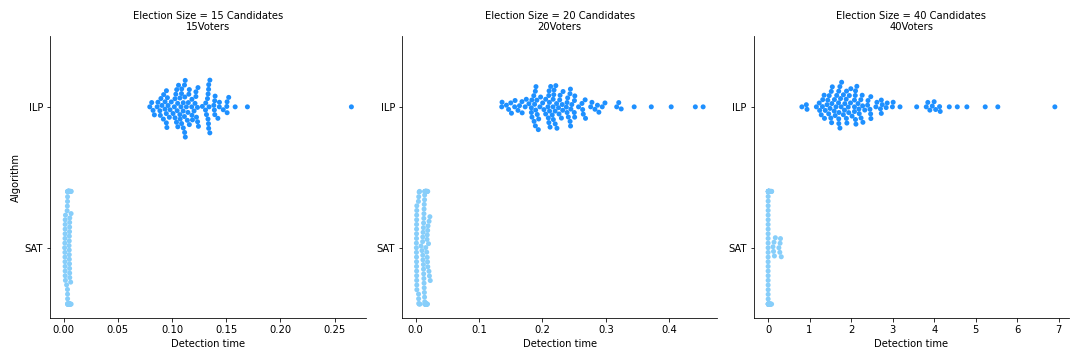
\includegraphics[width=\linewidth]{ex1-swarm.png}
    \centering
    \caption{Swarm Plot: VR (COP) Detection time comparison between ILP and SAT}
    \label{fig:detection:time:1}
\end{figure}

\begin{figure}[H]
    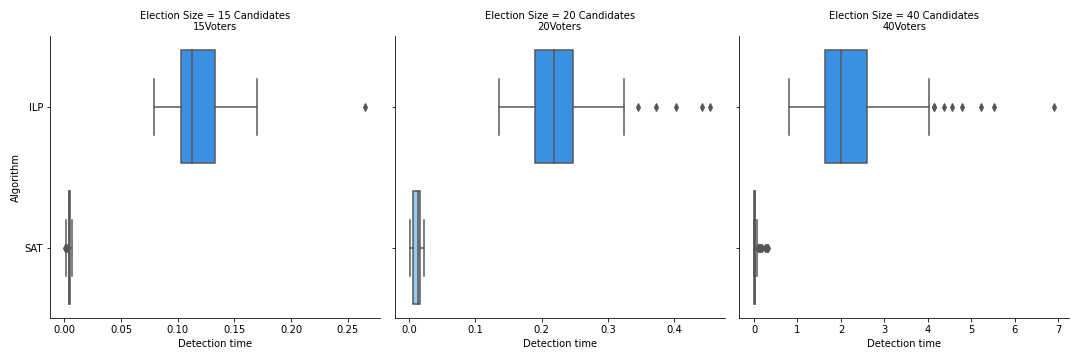
\includegraphics[width=\linewidth]{ex1-box.png}
    \centering
    \caption{Box Plot: VR (COP) Detection time comparison between ILP and SAT}
    \label{fig:detection:time:2}
\end{figure}

\begin{figure}[H]
    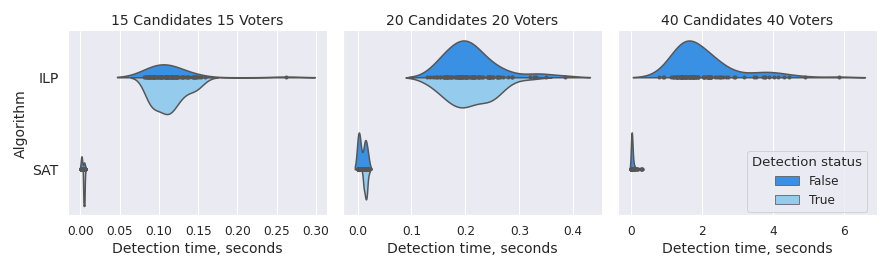
\includegraphics[width=\linewidth]{ex1-violin.png}
    \centering
    \caption{Violin Plot: VR (COP) Detection time comparison between ILP and SAT}
    \label{fig:detection:time:3}
\end{figure}